\documentclass[border=4pt]{standalone}
\usepackage{tikz}
\usetikzlibrary{positioning, arrows.meta, shapes.geometric, calc, fit, backgrounds}
\usepackage{amsmath,amssymb}
\begin{document}
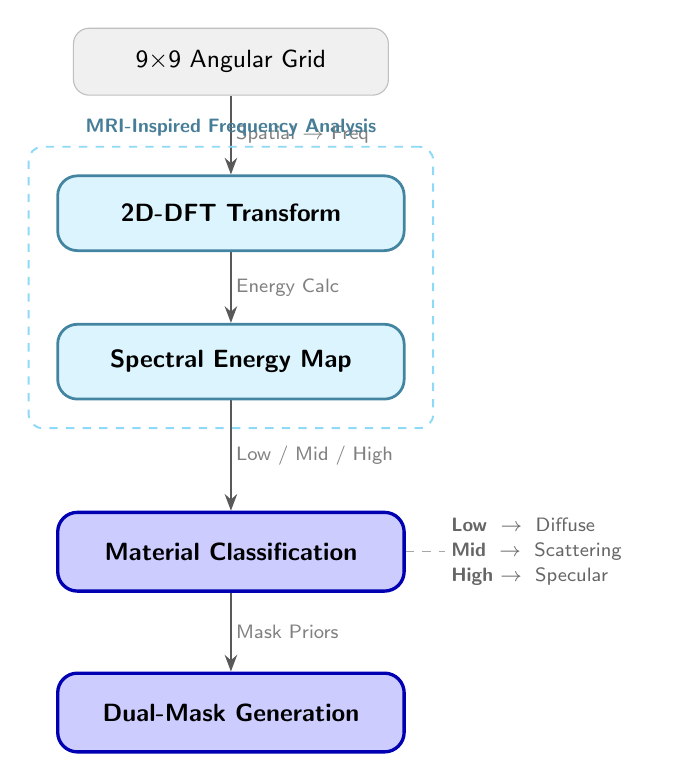
\begin{tikzpicture}[
  inp/.style={draw, rounded corners=2mm, minimum width=4.0cm, minimum height=0.85cm,
              fill=gray!12, draw=gray!50, align=center, font=\sffamily\small},
  freq/.style={draw, rounded corners=2.5mm, minimum width=4.4cm, minimum height=0.95cm,
               fill=cyan!14, draw=cyan!60!black, line width=1pt, align=center,
               font=\sffamily\small\bfseries},
  innov/.style={draw, rounded corners=2.5mm, minimum width=4.4cm, minimum height=1.0cm,
                fill=blue!20, draw=blue!70!black, line width=1.2pt, align=center,
                font=\sffamily\small\bfseries},
  arr/.style={-{Stealth[length=6pt]}, thick, color=black!65},
  lbl/.style={font=\sffamily\scriptsize, text=black!50, fill=white, inner sep=1.5pt},
  gbox/.style={draw=cyan!45, dashed, rounded corners=5pt, inner sep=10pt, line width=0.7pt},
  note/.style={font=\sffamily\scriptsize, text=black!60, align=left, inner sep=2pt},
  bandlbl/.style={font=\sffamily\scriptsize\bfseries, text=black!70},
]

% m1: Input - 9x9 Angular Grid
\node[inp] (m1) {9$\times$9 Angular Grid};

% m2: 2D-DFT Transform (inside group)
\node[freq, below=1.0cm of m1] (m2) {2D-DFT Transform};

% m3: Spectral Energy Map (inside group)
\node[freq, below=0.9cm of m2] (m3) {Spectral Energy Map};

% m4: Material Classification
\node[innov, below=1.4cm of m3] (m4) {Material Classification};

% m5: Dual-Mask Generation
\node[innov, below=1.0cm of m4] (m5) {Dual-Mask Generation};

% Main flow arrows on background layer
\begin{scope}[on background layer]
  \draw[arr] (m1) -- node[lbl, right] {Spatial $\to$ Freq} (m2);
  \draw[arr] (m2) -- node[lbl, right] {Energy Calc} (m3);
  \draw[arr] (m3) -- node[lbl, right] {Low / Mid / High} (m4);
  \draw[arr] (m4) -- node[lbl, right] {Mask Priors} (m5);
\end{scope}

% Group box around frequency analysis
\node[gbox, fit=(m2)(m3),
      label={[font=\sffamily\scriptsize\bfseries, text=cyan!55!black]above:MRI-Inspired Frequency Analysis}] (g1) {};

% Side annotation: frequency bands to material mapping
\node[note, right=0.5cm of m4, anchor=west, text width=2.7cm] (annot) {
  \textbf{Low} $\;\rightarrow\;$ Diffuse\\[1pt]
  \textbf{Mid} $\;\rightarrow\;$ Scattering\\[1pt]
  \textbf{High} $\rightarrow\;$ Specular
};

% Small dashed connector from annotation to m4
\draw[dashed, color=black!35, line width=0.5pt] (m4.east) -- (annot.west);

\end{tikzpicture}
\end{document}